\chapter*{Úvod}
\addcontentsline{toc}{chapter}{Úvod}

V~mnoha informatických oblastech se setkáváme s~potřebou vyjádřit nějakou časovou informaci. Ať už se pohybujeme na poli plánování, formální verifikace nebo paralelního programování, mohou se na naši práci vztahovat časová omezení, na která musíme brát zřetel. Není tedy divu, že s~postupným vývojem těchto disciplín roste potřeba pro efektivní způsoby, kterými bychom tato omezení mohli analyzovat.

Jedním z~nejzákladnějších a~nejběžnějších typů časových omezení jsou takzvaná \emph{rozdílová omezení}. Jak už napovídá jejich název, týkají se časového rozdílu mezi dvěma událostmi. Matematickým formalizmem bychom mohli rozdílové omezení definovat například ve tvaru $X_i - X_j \in [t_1, t_2]$ nebo ekvivalentně jako $X_i - X_j \leq t$. Vzhledem k~relativní jednoduchosti takové podmínky byl problém splnitelnosti konjunkce rozdílových omezení nazván \emph{simple temporal problem} (STP). Přes jejich zdánlivou přímočarost se ale rozdílová omezení ukázala jako dostatečně expresivní pro velkou řadu problémů. Uvažujme například následující situaci, jejíž paralely můžeme nalézt v~oblasti plánování: 

\begin{center}
\begin{minipage}{\textwidth}
Na strojích $s_1 \dots s_n$ potřebujeme provést celkem $m$ úkolů. Každý úkol se skládá z~nějakého množství operací. Každá operace musí proběhnout na konkrétním stroji a~zabere nějaký čas. Operace náležící témuž úkolu navíc musí proběhnout v~pevně daném pořadí. Dokážeme jednotlivé operace rozplánovat mezi všechny stroje tak, aby výpočet skončil před cílovým časem $T$?
\end{minipage}
\end{center}

Příklad převodu takového zadání do tvaru rozdílových omezení ukazuje obrázek \ref{fig:job}. Jistě není těžké představit si reálná využití pro řešení takového problému. Jak si ale můžeme všimnout, už se nejedná o~běžný STP --- v~problému se navíc objevují disjunkce omezení. Naše podmínky obecně odpovídají výrokové formuli (v~konjunktivní normální formě), jejíž atomy jsou rozdílová omezení. Problém splnitelnosti takovýchto formulí se obecně nazývá \emph{satisfiability modulo theories} (SMT) a~je důležitým předmětem zkoumání v~oboru formální verifikace \cite{SMT}. Přestože je tento problém obecně složitější než STP, ukážeme si, že jeho rozhodnutí jsme stále schopni dosáhnout vhodným využitím postupů na řešení STP.

\begin{figure}[b]
	\centering
	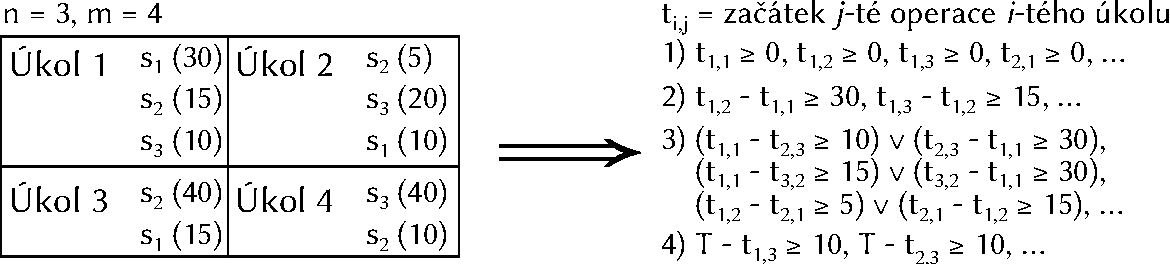
\includegraphics[width=\textwidth]{jobshop.pdf}
	\caption{Příklad převodu plánovacího problému do rozdílových omezení} 
	\label{fig:job}
\end{figure}

Cílem této práce je vytvoření STP řešiče pro verifikační framework OpenSMT \cite{OpenSMT}. Nejprve si přiblížíme některé základní principy z~oblasti SMT řešičů. Následně analyzujeme existující postupy pro řešení STP v~kontextu SMT a~navrhneme podle nich konkrétní algoritmus pro zapojení do OpenSMT. Navržený algoritmus následně implementujeme. Jako součást práce také naši implementaci otestujeme na rozsáhlé sadě problémů a~srovnáme její účinnost s~existujícími SMT řešiči.
